\chapter{QoS metrics}

If you go to the postal office to submit a packet, you will be offered different options.
In addition to the regular service, it is possible that an urgent service exists.
Probably there is also the possibility sending the packet as certified mail, and some option for delivery notification.
It is likely that there are also special services for packets that are voluminous or heavy.

QoS-enabled packet switched networks also offer different kinds of services for data packet delivery.
In this chapter, we will review the different metrics that are relevant for data networks.
This metrics can be used to establish \emph{service level agreements} (SLAs) which are contracts specifying the QoS expected from a network.
These contracts should also specify how the metrics are actually measured.

As an example, if a network guarantees a delay below 100 ms, it should be specified whether this makes reference to the maximum, the delay or the 95\% percentile.
The measures will also differ depending whether 5 minutes averages or 1 hour averages are considered.
This makes the specification of SLAs tricky.

\section{Delay}
Delay is the time that it is required to traverse the network from the entry point to the exit point.
Delay is normally considered for real-time services such as voice over IP (VoIP).
The total end-to-end delay is simply the sum of the delay suffered in each of the hops in the data network.
As an example, \ref{fig:four_hops} shows a network with four hops.

\begin{figure}[h]
\centering
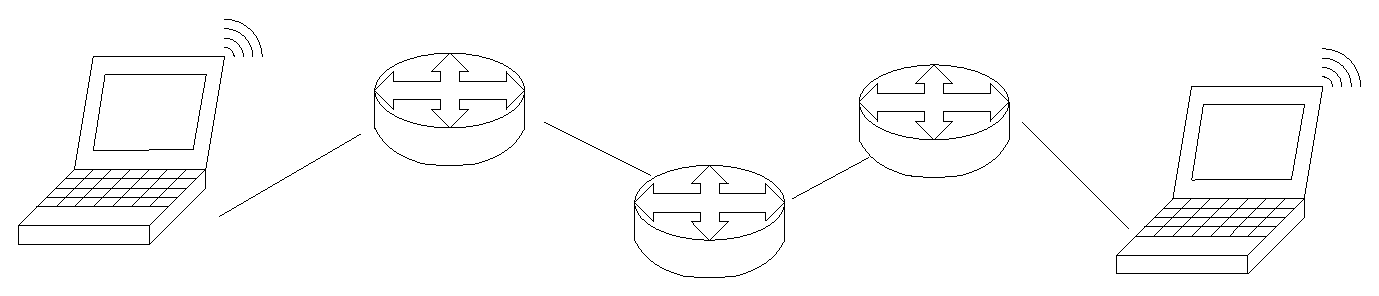
\includegraphics[width=\linewidth]{figures/four_hops.eps}
\caption{A network with two terminals, three routers and four hops.}
\label{fig:four_hops}
\end{figure}

In each hop, there are four different contributions to delay:
\begin{enumerate}
\item Processing: The time required for the router or switching device to put the packet on the outgoing interface queue.
Very short.
\item Queueing: Waiting time on the outgoing interface queue.
Very short if the queue is empty.
\item Transmission: The time required to put the packet on the transmission medium. It is a function of the packet length and transmission rate.
Short in high-speed transmission media.
\item Propagation: The time that it takes for the packet to travel the distance from the hop source to the hop destination.
Short time over short distances. 
And very long when it involves a trip to a geostationary satellite.
\end{enumerate}

